\subsection{Mallado}

\noindent
\justify

Gran parte del \'exito de las simulaciones num\'ericas recaen en la discretizaci\'on del dominio y en la calidad de los elementos que la componen. Se desarroll\'o una metodolog\'ia de mallado autom\'atico con base en el lenguaje \textit{gmsh} tomando como variables de entrada las dimensiones de la geometr\'ia definida en la secci\'on \ref{geo}. Esta metodolog\'ia emplea elementos de diferentes tama\~nos y permite tambi\'en definir su naturaleza (rectangulares o triangulares).

\noindent
\justify

El algoritmo ejecuta, adem\'as, un refinamiento autom\'atico en la zona en donde ocurre el mayor grado de sedimentaci\'on: en la superficie inclinada, como se aprecia en la Figura \ref{malla:geo}.

\begin{figure}[h!]
	\centering
	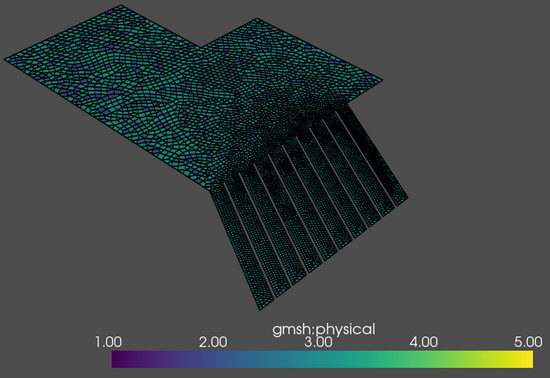
\includegraphics[width=\textwidth]{Images/CFDEM/malla2.png}
	\caption{Mallado de la geometr\'ia.}
	\label{malla:geo}
\end{figure}

\newpage

\noindent
\justify

La malla mostrada en la Figura \ref{malla:geo} presenta las siguientes caracter\'isticas:

\begin{table}[h!]
	\centering
	\begin{tabular}{|c|c|}
		\hline
		\textbf{Par\'ametro} & \textbf{Valor} \\ \hline
		Tipo de elementos & Rectangulares \\ \hline
		N\'umero de elementos & 20415 \\ \hline
		N\'umero de nodos & 13692 \\ \hline	
	\end{tabular}
	\caption{Datos de la malla generada.}
	\label{malla}
\end{table}

\noindent
\justify

Al emplear el m\'etodo \texttt{checkMesh} de OpenFOAM para el an\'alisis preliminar de malla, se obtuvieron los siguientes resultados:

\begin{table}[h!]
	\centering
	\begin{tabular}{|c|c|}
		\hline
		\textbf{Par\'ametro} & \textbf{Valor} \\ \hline
		Apertura \textit{m\'axima} entre elementos & 11.45 \\ \hline
		Checkeo de \textit{no} ortogonalidad & OK \\ \hline
		Oblicuidad m\'axima & 0.66 OK \\ \hline
		Conclusi\'on de malla & OK \\ \hline
	\end{tabular}
	\caption{Resumen de resultados sobre el checkeo de malla.}
	\label{check}
\end{table}

\noindent
\justify

A partir de los resultados mostrados en el Cuadro \ref{check}, se concluye que la malla es \'optima para el desarrollo de las simulaciones num\'ericas consecutivas.